\documentclass{article}
\usepackage[utf8]{inputenc}
\usepackage[margin=1.2in]{geometry}
\usepackage{hyperref}

\PassOptionsToPackage{usenames,dvipsnames,svgnames}{xcolor}  
\usepackage{tikz}
\usetikzlibrary{arrows,positioning,automata}

\usepackage{natbib}
\usepackage{graphicx}
\usepackage{amsmath}
\usepackage{listings}
\usepackage{xcolor}


\definecolor{codegreen}{rgb}{0,0.6,0}
\definecolor{codegray}{rgb}{0.5,0.5,0.5}
\definecolor{codepurple}{rgb}{0.58,0,0.82}
\definecolor{backcolour}{rgb}{0.95,0.95,0.92}
\definecolor{deepblue}{rgb}{0,0,0.5}
\definecolor{deepred}{rgb}{0.6,0,0}
\definecolor{deepgreen}{rgb}{0,0.5,0}

\lstdefinestyle{mystyle}{
    backgroundcolor=\color{white},   
    commentstyle=\color{codegreen},
    keywordstyle=\color{deepblue},
    numberstyle=\tiny\color{codegray},
    stringstyle=\color{deepgreen},
    emph={Agent,__init__,act,self,union,exists, scope},
    emphstyle=\color{deepred},
    basicstyle=\ttfamily\footnotesize,
    breakatwhitespace=false,         
    breaklines=true,                 
    captionpos=b,                    
    keepspaces=true,                 
    numbers=left,                    
    numbersep=5pt,                  
    showspaces=false,                
    showstringspaces=false,
    showtabs=false,                  
    tabsize=3
}

\lstset{style=mystyle}

\title{\vspace{-2 cm} Universidade Federal de Ouro Preto \\ BCC 325 - Inteligência Artificial \\ Prova 2 \\ Prof. Rodrigo Silva}
\date{}


\begin{document}

\maketitle

\vspace{0.4 cm}
\begin{enumerate}


%Regressão Linear

\item Para se obter os pesos, $\mathbf{w}$, de um modelo de regressão linear utilizamos a expressão  $\mathbf{w} = (X^{t}X)^{-1}X^t\mathbf{y}$. Considerando a seguinte base de dados, responda:

\begin{table}[h!]
    \footnotesize
    \centering
    \begin{tabular}{|c|c|c|}
    \hline
    \textbf{Atributo1} & \textbf{Atributo2} & \textbf{Classe} \\
    \hline
    1.2 & 2 & 3 \\
    2.3 & 3 & 5 \\
    3.5 & 4 & 6 \\
    4   & 5 & 8 \\
    5.7 & 2 & 2 \\
    6.7 & 2.5 & 9 \\
    \hline
    \end{tabular}
    \label{tab:exemplo}
\end{table}


\begin{enumerate}
    \item Defina $X$ em termos da base de dados apresentada. Considere a necessidade de determinar a constante que representa a interceptação do modelo com o eixo vertical.
    \item Defina o vetor $\mathbf{y}$ em termos da base dados apresentada.
    \item Explique como a equação $\mathbf{w} = (X^{t}X)^{-1}X^t\mathbf{y}$ é obtida.
    \item É possivel utilizar este método para resolver problemas em que a relação entre variável dependente (atributo alvo), $y$, e as variáveis independentes (atributos de entrada), $\mathbf{x}$, não é linear? Como?
    \item Apresente $X$ para o caso em que suspeitamos que a relação entre $\mathbf{x}$ e $y$ é quadrática.
\end{enumerate}

\item Considere os dados abaixo:

    \begin{figure}[!hb]
        \centering
        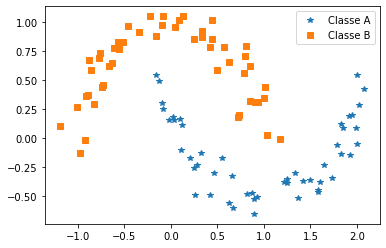
\includegraphics[width=0.41\textwidth]{moons.png}
    \end{figure}
    
    \begin{enumerate}
        \item Qua tipo de problema resolvemos com regressão logística?
        \item É possível resolver este problema com um aplicação direta do algoritmo de regresão logística com as variáveis definidas nos eixos \textit{x} e \textit{y}? Por quê?
        \item O que poderia ser feito para que este problema seja resolvível com regressão logística?
        \item Como o vetor de pesos $\mathbf{w}$ é obtido quanto temos um modelo de regressão logística? 
    \end{enumerate}

\item Quando dizemos que um algoritmo de aprendizado de máquina ``está aprendendo'', que processo algorítmico está acontecendo?

\item Considere a base de dados abaixo:

\begin{table}[ht!]
    \footnotesize
    \centering
    \begin{tabular}{|c|c|c|}
    \hline
    \textbf{Atributo1} & \textbf{Atributo2} & \textbf{Classe} \\
    \hline
    1 & 2 & Classe1 \\
    2 & 3 & Classe1 \\
    3 & 4 & Classe2 \\
    4 & 5 & Classe2 \\
    5 & 20 & Classe1 \\
    6 & 30 & Classe1 \\
    7 & 40 & Classe2 \\
    8 & 50 & Classe2 \\
    \hline
    \end{tabular}
    \label{tab:dados_arvore}
    \end{table}

\begin{enumerate}
    \item Calcule o gini para a condição $Atributo1 \leq 4.5$. $I_{G}(p) = 1 - \sum_{i=1}^{J} p_{i}^{2}$
    \item Quais seriam condições ótimas, em relação ao gini, após selecionarmos como raíz da árvore de decisão o critério $Atributo1 \leq 4.5$. Desenhe essa árvore.
\end{enumerate}

\item O que é overfitting? Quais são os indícios de que um modelo está sofrendo de overfitting? De forma geral, o que deve ser feito para diminuir o overfitting?

\item Quais as vantagens do algoritmo de busca em largura sobre o algoritmo de busca em profundidade? E quais as desvantagens?

\item Quando devemos utilizar o algoritmo de busca A*?


\end{enumerate}

\end{document}

